\documentclass[a4paper,14pt]{extarticle}
\usepackage{../../tex-shared/report-layout}

\renewcommand{\mylabnumber}{2}
\renewcommand{\mylabtitle}{Исследование и функциональное моделирование процессов при помощи методологии IDEF0 с использованием CASE-средства поддержки методологии функционального моделирования процессов}
\renewcommand{\mysubject}{Методы и средства проектирования информационных систем}
\renewcommand{\mylecturer}{Заикина Е.Н.}

\begin{document}
\begin{titlepage}
    
    \thispagestyle{empty}
    
    \begin{center}
        
        Министерство науки и Высшего образования Российской Федерации \\
        Севастопольский государственный университет \\
        Кафедра ИС
        
        \vfill

        Отчет \\
        по лабораторной работе №\mylabnumber \\
        \enquote{\mylabtitle} \\
        по дисциплине \\
        \enquote{\MakeTextUppercase{\mysubject}}

    \end{center}

    \vspace{1cm}

    \noindent\hspace{7.5cm} Выполнил студент группы ИС/б-17-2-о \\
    \null\hspace{7.5cm} Горбенко К. Н. \\
    \null\hspace{7.5cm} Проверил \\
    \null\hspace{7.5cm} \mylecturer

    \vfill

    \begin{center}
        Севастополь \\
        \the\year{}
    \end{center}

\end{titlepage}

\section{Цель работы}
\begin{itemize}
    \item осуществить исследование и функциональное моделирование процессов при
          помощи IDEF0-диаграмм;
    \item осуществить выбор и применение инструментального средства
          функционального моделирования процессов (IDEF0 диаграммы).
\end{itemize}

\section{Ход работы}
Составим контекстную диаграмму основного процесса (\ref{fig:context-diagram}) в
нотации \code{IDEF0}.

\begin{figure}[H]
    \centering
    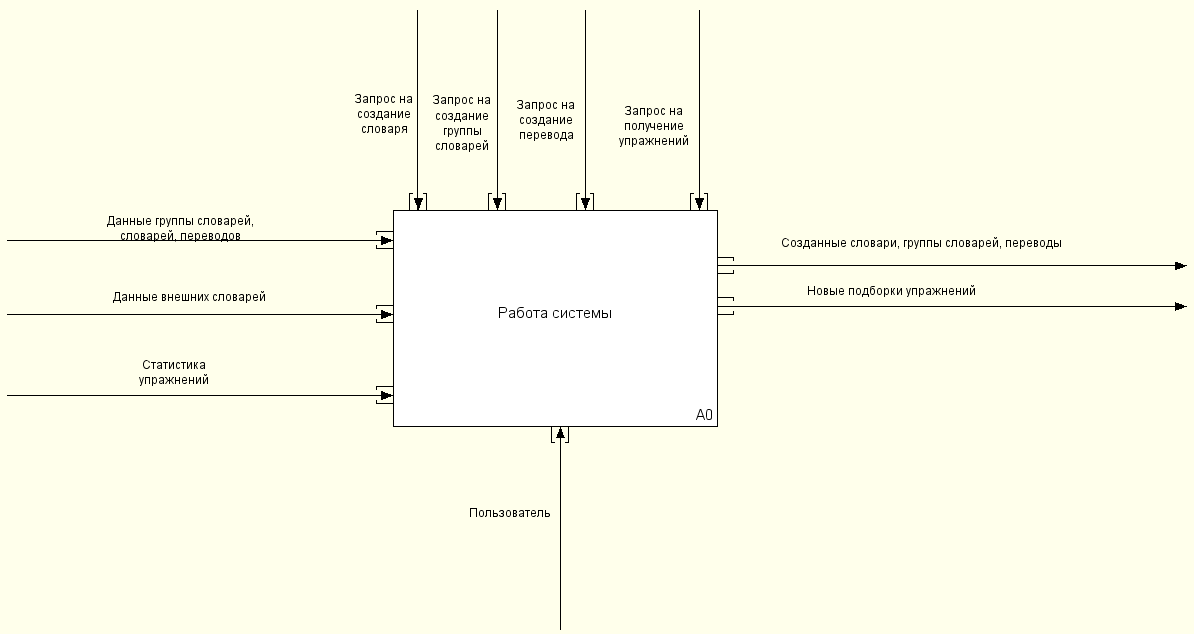
\includegraphics[width=\linewidth]{context-diagram}
    \caption{Контекстная диаграмма основного процесса системы}
    \label{fig:context-diagram}
\end{figure}

На рисунке \ref{fig:tree} изображена диаграмма дерева узлов системы.
\begin{figure}[H]
    \centering
    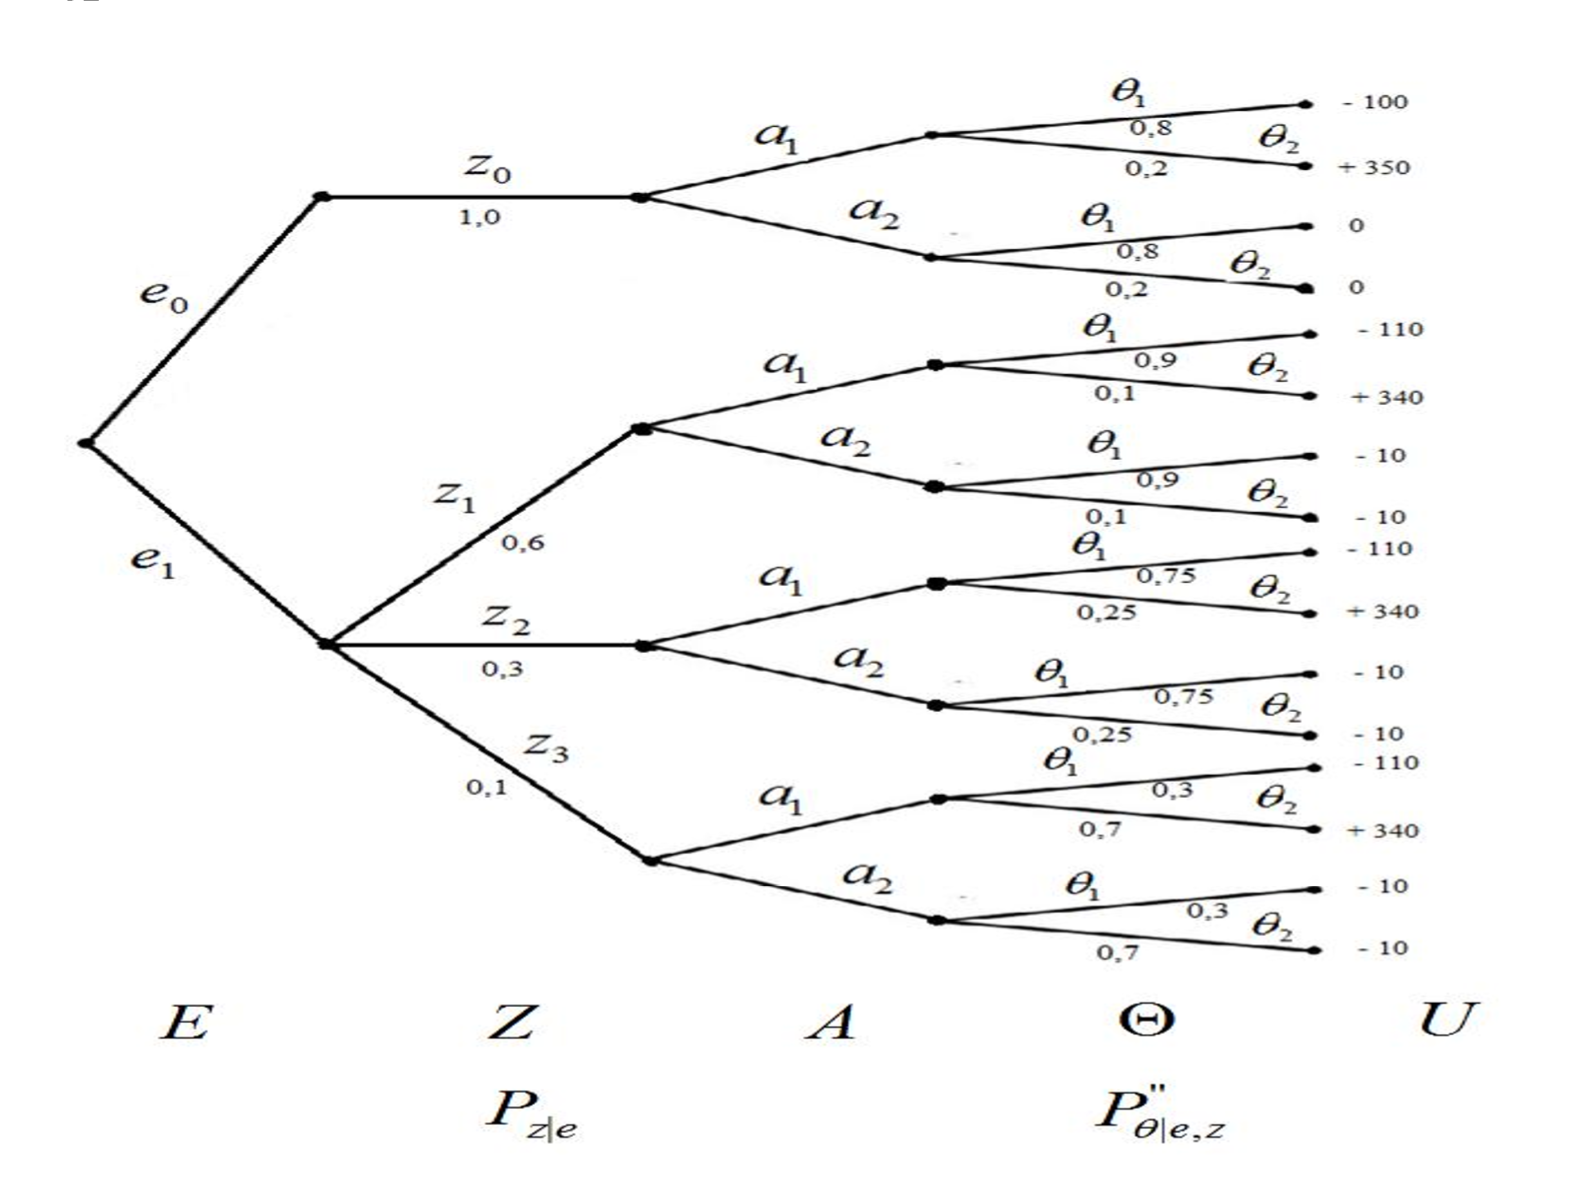
\includegraphics[width=\linewidth]{tree}
    \caption{Диаграмма дерева узлов системы}
    \label{fig:tree}
\end{figure}

Детализируем основной процесс системы, изображенный на рисунке
\ref{fig:context-diagram}. Результат изображен на рисунке \ref{fig:detailed-main-process}.

\begin{figure}[H]
    \centering
    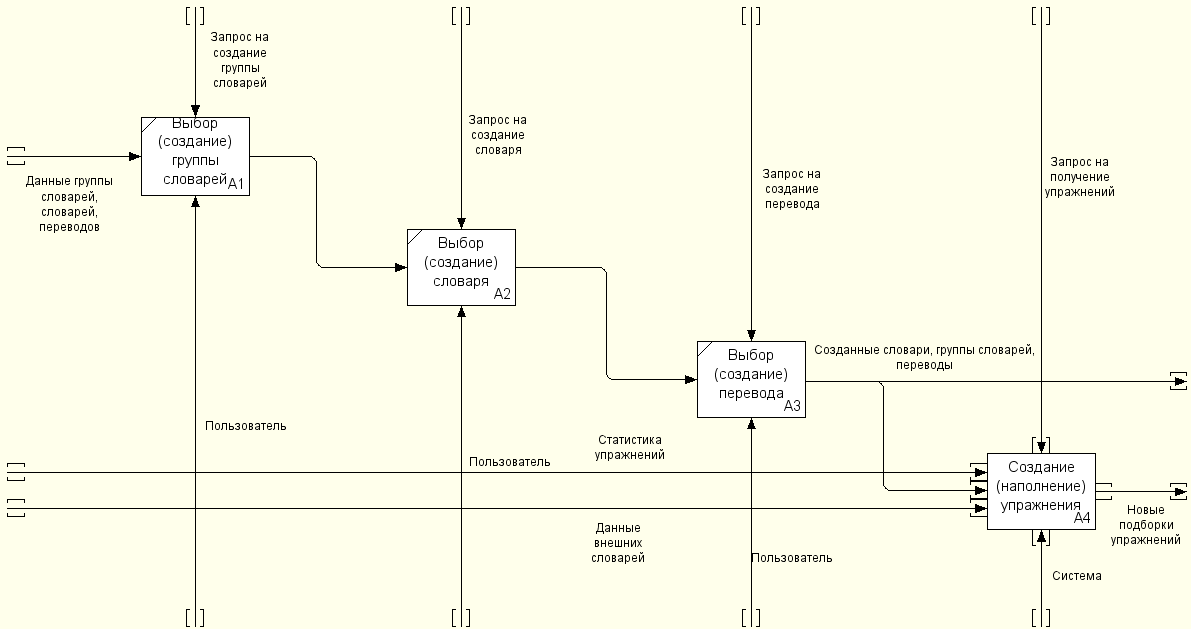
\includegraphics[width=\linewidth]{detailed-main-process}
    \caption{Детализированный основной процесс}
    \label{fig:detailed-main-process}
\end{figure}

Далее детализируем процесс создания упражнений \ref{fig:detailed-excercise-receival-process}:
\begin{figure}[H]
    \centering
    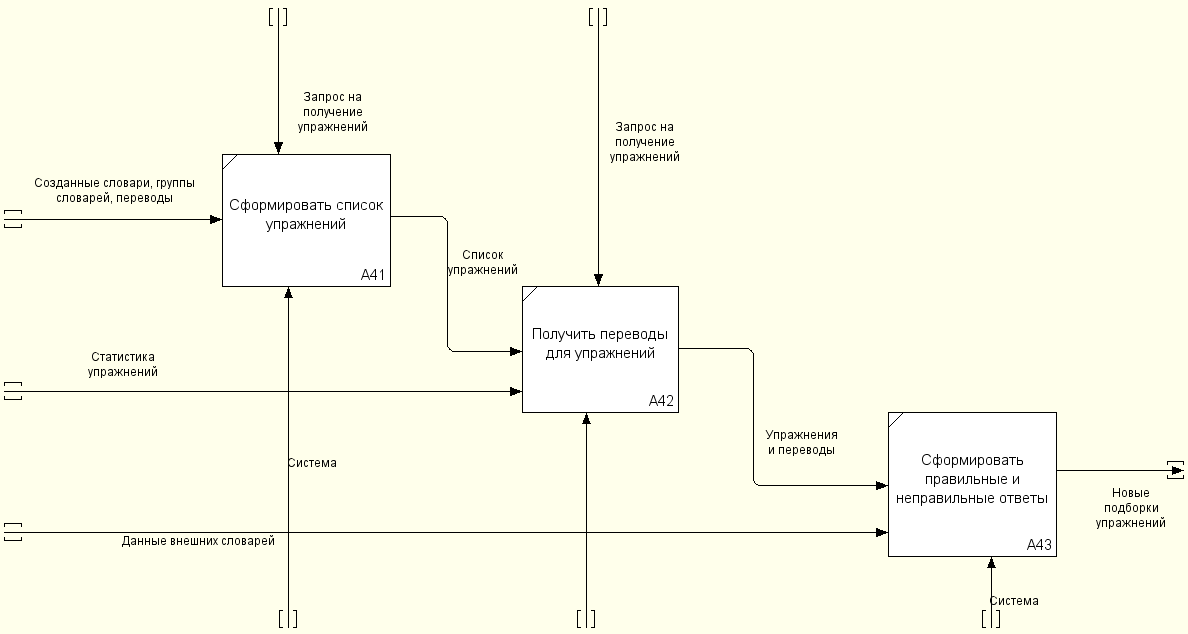
\includegraphics[width=\linewidth]{detailed-excercise-receival-process}
    \caption{Детализированный процесс создания упражнений}
    \label{fig:detailed-excercise-receival-process}
\end{figure}

\section*{Выводы}
В ходе лабораторной работы было осуществлено исследование и функциональное
моделирование процессов системы изучения лексики иностранного языка при помощи
\code{IDEF0}-диаграмм с помощью системы функционального моделирования
\code{Ramus Educational}.

\end{document}